\documentclass[10pt, aspectratio=169,usenames,dvipsnames]{beamer}

\usepackage{clases}

\title{Investigación Operativa}
\subtitle{Problema Dual}
\date{}
\author{Nazareno Faillace Mullen}
% \institute{Center for modern beamer themes}
% \titlegraphic{\hfill\includegraphics[height=1.5cm]{logo.pdf}}

\begin{document}

\maketitle

\begin{frame}{Dualidad - Motivación}
Cada problema lineal tiene asociado un problema dual. Entre ellos existe una conexión que da lugar a una serie de propiedades interesantes.
\vskip 0.5cm
El planteo del problema dual puede surgir a partir de la necesidad de encontrar cotas para el valor óptimo de nuestro problema.
\end{frame}

\begin{frame}{Dualidad - Motivación}
Por ejemplo, si tenemos el siguiente problema:
\[
\begin{array}{rrl}
    \max & \multicolumn{2}{l}{z=3x_1 + 2x_2}  \\
    \textit{s.a:} & x_1+3x_2 \leq & 5 \\
     & 6x_1-x_2 \leq & 18 \\
     & x_1 + 2x_2 \leq & 4 \\
     & x_1,x_2 \geq & 0
\end{array}
\]
Nos podría interesar hallar una cota superior para el valor óptimo $\zopt$. La idea es manipular las restricciones para lograr una desigualdad que permita acotar $\zopt$.
\vskip 0.5cm

\end{frame}

\begin{frame}{Dualidad - Motivación}
    \small
    \textbf{Idea:}\\
    
    Consideramos las variables $y_1, y_2, y_3\geq 0$ tales que:
    \[
    \begin{array}{rl}
    (x_1+3x_2)y_1 \leq & 5y_1 \\
    (6x_1-x_2)y_2 \leq & 18y_2 \\
    (x_1 + 2x_2)y_3 \leq & 4y_3 \\
    \end{array}
    \Rightarrow
    \begin{array}{rl}
    x_1y_1+3x_2y_1 \leq & 5y_1 \\
    6x_1y_2-x_2y_2 \leq & 18y_2 \\
    x_1y_3 + 2x_2y_3 \leq & 4y_3 \\
    \end{array}
    \]
    Si sumamos las tres desigualdades, tenemos que:
    \[(y_1+6y_2+y_3)x_1+(3y_1-y_2+2y_3)x_2 \leq 5y_1+18y_2+4y_3 \]
    Ahora, como nos gustaría que el lado izquierdo de la desigualdad acote a $z$, tenemos que pedir las siguientes condiciones:
    \[ y_1+6y_2+y_3 \geq 3 \qquad (1) \]
    \[ 3y_1-y_2+2y_3 \geq 2 \qquad (2)\]
    Es decir, si se cumplen ambas condiciones, tenemos que:
    \[z=3x_1+2x_2\overset{\text{(1) y (2)}}\leq(y_1+6y_2+y_3)x_1+(3y_1-y_2+2y_3)x_2 \leq 5y_1+18y_2+4y_3 \]
    Luego, para cualesquiera $y_1,y_2,y_3\geq0$ que cumplan (1) y (2), podemos armarnos una cota para $z$
\end{frame}

\begin{frame}{Dualidad}
    Como el problema primal tiene como objetivo \alert{maximizar}, nos interesa la mejor \alert{cota superior} para $z$, entonces, el problema dual se plantea como:
    \[
    \begin{array}{rrl}
        \min & \multicolumn{2}{l}{5y_1+18y_2+4y_3} \\
        \text{s.a:} & y_1+6y_2+y_3 \geq & 3 \\
        & 3y_1-y_2+2y_3 \geq & 2 \\
        & y_1,y_2,y_3\geq & 0
    \end{array}
    \]
    \pause
    \begin{tcolorbox}[colback=blue!25, colframe=blue!55!white]
    \textbf{Observación 1}:\\
    $\#$ Variables del primal = $\#$ Restricciones del dual \\
    $\#$ Restricciones del primal = $\#$ Variables del dual
    \end{tcolorbox}
\end{frame}

\begin{frame}{}
%    En general, las formulaciones del problema primal y del problema dual se relacionan de la siguiente
%    manera:
    \vspace{2em}
    \begin{columns}
        \begin{column}{0.5\textwidth}
    \begin{adjustbox}{width = \textwidth}
    \begin{tabular}{|l|l|} \hline
        \multicolumn{1}{|c|}{Primal} & \multicolumn{1}{c|}{Dual}  \\ \hline
        Obj: Minimizar & Obj: Maximizar \\ \hline
        % Obj: Minimizar & Obj: Maximizar \\ \hline
        $\imath$-ésima restricción $\leq$ & $\imath$-ésima variable $\leq 0$ \\
        $\imath$-ésima restricción $\geq$ & $\imath$-ésima variable $\geq 0$ \\
        $\imath$-ésima restricción $=$ & $\imath$-ésima variable libre \\
        $\jmath$-ésima variable $\geq 0$ & $\jmath$-ésima restricción $\leq$ \\
        $\jmath$-ésima variable $\leq 0$ & $\jmath$-ésima restricción $\geq$ \\
        $\jmath$-ésima variable libre & $\jmath$-ésima restricción $=$ \\ \hline
    \end{tabular}
    \end{adjustbox}
    \end{column}
    \begin{column}{0.5\textwidth}
    \begin{adjustbox}{width = \textwidth}
    \begin{tabular}{|l|l|} \hline
        \multicolumn{1}{|c|}{Primal} & \multicolumn{1}{c|}{Dual}  \\ \hline
        Obj: Maximizar & Obj: Minimizar \\ \hline
        % Obj: Minimizar & Obj: Maximizar \\ \hline
        $\imath$-ésima restricción $\leq$ & $\imath$-ésima variable $\geq 0$ \\
        $\imath$-ésima restricción $\geq$ & $\imath$-ésima variable $\leq 0$ \\
        $\imath$-ésima restricción $=$ & $\imath$-ésima variable libre \\
        $\jmath$-ésima variable $\geq 0$ & $\jmath$-ésima restricción $\geq$ \\
        $\jmath$-ésima variable $\leq 0$ & $\jmath$-ésima restricción $\leq$ \\
        $\jmath$-ésima variable libre & $\jmath$-ésima restricción $=$ \\ \hline
    \end{tabular}
    \end{adjustbox}
    \end{column}
    \end{columns}

    \textbf{Ejercicio}: hallar el dual asociado al siguiente problema:
    \[
    \begin{array}{rrl}
        \max & \multicolumn{2}{l}{3x_1+2x_2-3x_3+4x_4}  \\
        \text{s.a:} & x_1-2x_2+3x_3+4x_4 \leq & 3 \\
         & x_2+3x_3+4x_4 \geq & 5 \\
         & 2x_1-3x_2-7x_3-4x_4 = & 2 \\
         & x_1 \geq & 0 \\
         & x_4 \leq & 0 \\
         & x_2, x_3 & \text{libres}
    \end{array}
    \]
    
\end{frame}

\begin{frame}{}
    \[
    \begin{array}{rrl}
        \max & \multicolumn{2}{l}{3x_1+2x_2-3x_3+4x_4}  \\
        \text{s.a:} & x_1-2x_2+3x_3+4x_4 \leq & 3 \\
         & x_2+3x_3+4x_4 \geq & 5 \\
         & 2x_1-3x_2-7x_3-4x_4 = & 2 \\
         & x_1 \geq & 0 \\
         & x_4 \leq & 0 \\
         & x_2, x_3 & \text{libres}
    \end{array}
    \]
    Notemos que:
    \begin{itemize}
        \item El primal tiene 4 variables $\Rightarrow$ El dual tendrá 4 restricciones
        \item El primal tiene 3 restricciones $\Rightarrow$ El dual tendrá 3 variables
    \end{itemize}
\end{frame}

%\begin{noheadline}
\begin{frame}{}
%    \footnotesize
    \[
    \begin{array}{rrrrrrrrrr}
        \text{\textcolor<10>{Periwinkle}{$\max$}} & \text{\textcolor<2>{Green}{3}}x_1&+&\text{\textcolor<3>{Green}{2}}x_2& \text{\textcolor<4>{Green}{-}}&\text{\textcolor<4>{Green}{3}}x_3&+&\text{\textcolor<5>{Green}{4}}x_4  \\
        \text{s.a:} & \only<2>{\text{\textcolor<2>{red}{1}}}x_1&\text{\textcolor<3>{red}{-}}&\text{\textcolor<3>{red}{2}}x_2&+&\text{\textcolor<4>{red}{3}}x_3&+&\text{\textcolor<5>{red}{4}}x_4 & \text{\textcolor<6>{JungleGreen}{$\mathbf{\leq}$}} & \text{\textcolor<10>{RubineRed}{3}} \\
         & \only<2>{\text{\textcolor{red}{0}}x_1} & \only<2>{+} & \only<3>{\text{\textcolor<3>{red}{1}}}x_2&+&\text{\textcolor<4>{red}{3}}x_3&+&\text{\textcolor<5>{red}{4}}x_4& \text{\textcolor<7>{JungleGreen}{$\mathbf{\geq}$}} & \text{\textcolor<10>{RubineRed}{5}} \\
         & \text{\textcolor<2>{red}{2}}x_1 & \text{\textcolor<3>{red}{-}} &\text{\textcolor<3>{red}{3}}x_2 & \text{\textcolor<4>{red}{-}} &\text{\textcolor<4>{red}{7}}x_3 & \text{\textcolor<5>{red}{-}} &\text{\textcolor<5>{red}{4}}x_4 & \text{\textcolor<8>{JungleGreen}{$\mathbf{=}$}} & \text{\textcolor<10>{RubineRed}{2}} \\
         & & & & & & &\text{\textcolor<2>{NavyBlue}{$x_1$}}& \text{\textcolor<2>{NavyBlue}{$\geq$}} & \text{\textcolor<2>{NavyBlue}{0}} \\
         & & & & & & &\text{\textcolor<5>{NavyBlue}{$x_4$}}& \text{\textcolor<5>{NavyBlue}{$\leq$}} & \text{\textcolor<5>{NavyBlue}{0}} \\
         & & & & & & & \text{\textcolor<3>{NavyBlue}{$x_2$}}, \text{\textcolor<4>{NavyBlue}{$x_3$}} & & \text{\textcolor<3-4>{NavyBlue}{libres}} \\
    \end{array}
    \]

    \begin{columns}
        \begin{column}{0.5\textwidth}
            \textbf{Restricciones:}
            \begin{center}
                \only<2>{\textcolor{red}{1}$y_1$+\textcolor{red}{0}$y_2$+\textcolor{red}{2}$y_3$ \textcolor{NavyBlue}{$\geq$} \textcolor{Green}{3}}
            \onslide<3->{$y_1+2y_3 \geq 3$}

            \only<3>{\begin{center}\textcolor<3>{red}{-2}$y_1$ + \textcolor<3>{red}{1}$y_2$ \textcolor<3>{red}{-3}$y_3$ \textcolor{NavyBlue}{=} \textcolor{Green}{2}\end{center}}
            \onslide<4->{$-2y_1+y_2-3y_3=2$}

            \only<4>{\begin{center} \textcolor<4>{red}{3}$y_1$ + \textcolor<4>{red}{3}$y_2$  \textcolor<4>{red}{-7}$y_3$ \textcolor{NavyBlue}{=} \textcolor{Green}{-3}\end{center}}
            \onslide<5->{$3y_1+3y_2-7y_3=-3$}

            \only<5>{\begin{center}
                \textcolor<5>{red}{4}$y_1$ + \textcolor<5>{red}{4}$y_2$ \textcolor<5>{red}{-4} $y_3$ \textcolor{NavyBlue}{$\leq$} \textcolor{Green}{4}
            \end{center}}
            \onslide<6->{$4y_1+4y_2-4y_3\leq 4$}
            \end{center}
        \end{column}
        \begin{column}{0.5\textwidth}
            \onslide<6->{\textbf{Variables:}}\\
            \begin{center}
            \only<6>{$y_1$ \textcolor{JungleGreen}{$\geq 0$}}
            \onslide<7->{$y_1\geq 0\quad$}
            \only<7>{$y_2$ \textcolor{JungleGreen}{$\leq 0$}}
            \onslide<8->{$y_2\leq 0\quad$}
            \only<8>{$y_3$ \textcolor{JungleGreen}{libre}}
            \onslide<9->{$y_3$ libre}
            \end{center}

            \onslide<10->{\textbf{Objetivo: }}\\
            \begin{center}
            \only<10>{\textcolor{Periwinkle}{$\min$} \text{\textcolor<10>{RubineRed}{3}}$y_1$ + \text{\textcolor<10>{RubineRed}{5}}$y_2$ + \text{\textcolor<10>{RubineRed}{2}}$y_3$}
            \onslide<11->{$\min \quad 3y_1+5y_2+2y_3$}
            \end{center}
        \end{column}
    \end{columns}

\end{frame}
%\end{noheadline}

\begin{frame}{}
    Primal:
        \[
    \begin{array}{rrl}
        \max & \multicolumn{2}{l}{3x_1+2x_2-3x_3+4x_4}  \\
        \text{s.a:} & x_1-2x_2+3x_3+4x_4 \leq & 3 \\
         & x_2+3x_3+4x_4 \geq & 5 \\
         & 2x_1-3x_2-7x_3-4x_4 = & 2 \\
         & x_1 \geq & 0 \\
         & x_4 \leq & 0
    \end{array}
    \]
    Dual:
    \[
    \begin{array}{rrl}
        \min & 3y_1+5y_2+2y_3 \\
        \text{s.a:} & y_1+2y_3 \geq & 3 \\
         & -2y_1+y_2-3y_3 = & 2 \\
         & 3y_1+3y_2-7y_3= & -3 \\
         & 4y_1+4y_2-4y_3 \leq & 4 \\
         & y_1\geq & 0 \\
         & y_2\leq & 0 \\
         & y_3 & \text{libre}
    \end{array}\]
\end{frame}

\begin{frame}{}
% \small
\vspace{1em}
\begin{tcolorbox}[title=Teorema débil de dualidad]
Para un problema con objetivo de maximizar, sean $(x_1,\cdots,x_n)$ solución factible del primal e $(y_1,\cdots, y_m)$ solución factible del dual, entonces:
\[ \displaystyle \sum_{j=1}^n c_jx_j \leq \sum_{i=1}^m b_iy_i\]
\footnotesize{\textbf{Obs:} si el objetivo del primal es minimizar, la desigualdad se invierte.}
\end{tcolorbox}

\begin{tcolorbox}[title= Teorema fundamental de dualidad]
Si el problema primal tiene solución óptima $(x_1^{\ast},\cdots,x_n^{\ast})$, entonces el dual tiene solución óptima $(y_1^{\ast},\cdots,y_m^{\ast})$ tal que:
\[ \displaystyle \sum_{j=1}^n c_jx_j^{\ast} = \sum_{i=1}^m b_iy_i^{\ast}\]
\end{tcolorbox}
\end{frame}


\begin{frame}{Dualidad - Teorema fundamental de dualidad}
    Los teoremas de dualidad nos permiten observar otra relación muy importante entre el problema primal y el problema dual:\\
    \begin{center}
    \begin{tabular}{|c|c|c|c|c|}
        \cline{3-5}
        \multicolumn{2}{c|}{} & \multicolumn{3}{c|}{Dual} \\\cline{3-5}
        \multicolumn{2}{c|}{} & Óptimo & Infactible & No acotado \\\hline
        \multirow{3}{*}{Primal} & Óptimo & \ding{51} & \ding{55} & \ding{55}\\ \cline{2-5}
         & Infactible & \ding{55} & \ding{51} & \ding{51} \\ \cline{2-5}
         & No acotado & \ding{55} & \ding{51} & \ding{55} \\\hline
    \end{tabular}\\
    \footnotesize{\ding{51}: puede ocurrir $\qquad$ \ding{55}: no puede ocurrir}
    \end{center}
\end{frame}

\begin{frame}{Dualidad - Teorema de Holgura Complementaria)}
    \begin{tcolorbox}[title= Teorema de Holgura Complementaria (THC)]
    Sean $\xopt=(x_1^{\ast},\cdots,x_n^{\ast})$ solución del primal e $\yopt=(y_1^{\ast},\cdots,y_m^{\ast})$ solución del dual, las siguientes son condiciones necesarias y suficientes para la optimalidad simultánea de $\xopt$ e $\yopt$:
    \[
    \begin{array}{ccccc}
        \displaystyle \sum_{i=1}^m a_{ij}\yopt_i=c_j & \text{o} & \xopt_j = 0 & \; \text{(o ambos)} \quad & \forall j=1,\cdots,n  \\
        \displaystyle \sum_{j=1}^m a_{ij}\xopt_j=b_i & \text{o} & \yopt_i = 0 & \; \text{(o ambos)} \quad & \forall i=1,\cdots,m  \\
    \end{array} \]
    \end{tcolorbox}
\end{frame}

\begin{frame}{}
    El THC nos permite calcular el óptimo del primal a partir del óptimo del
    dual (y viceversa).\\
    \vskip 0.5cm
    \textbf{Ejemplo:} resolver el siguiente problema lineal:
    $$
    \begin{array}{rrl}
    \max & \multicolumn{2}{l}{2x_1+2x_2+\frac{3}{2}x_3}\\
    \text{s.a:}& 2x_1+x_2+\frac{1}{2}x_3\leq & 18\\
     & x_1+2x_2+3x_3\leq & 15\\
     & x_1, x_2, x_3\geq & 0 \\
    \end{array}
    $$
    \only<1>{
   \begin{columns}
        \begin{column}{0.5\textwidth}
    \begin{adjustbox}{width = \textwidth}
    \begin{tabular}{|l|l|} \hline
        \multicolumn{1}{|c|}{Primal} & \multicolumn{1}{c|}{Dual}  \\ \hline
        Obj: Minimizar & Obj: Maximizar \\ \hline
        % Obj: Minimizar & Obj: Maximizar \\ \hline
        $\imath$-ésima restricción $\leq$ & $\imath$-ésima variable $\leq 0$ \\
        $\imath$-ésima restricción $\geq$ & $\imath$-ésima variable $\geq 0$ \\
        $\imath$-ésima restricción $=$ & $\imath$-ésima variable libre \\
        $\jmath$-ésima variable $\geq 0$ & $\jmath$-ésima restricción $\leq$ \\
        $\jmath$-ésima variable $\leq 0$ & $\jmath$-ésima restricción $\geq$ \\
        $\jmath$-ésima variable libre & $\jmath$-ésima restricción $=$ \\ \hline
    \end{tabular}
    \end{adjustbox}
    \end{column}
    \begin{column}{0.5\textwidth}
    \begin{adjustbox}{width = \textwidth}
    \begin{tabular}{|l|l|} \hline
        \multicolumn{1}{|c|}{Primal} & \multicolumn{1}{c|}{Dual}  \\ \hline
        Obj: Maximizar & Obj: Minimizar \\ \hline
        % Obj: Minimizar & Obj: Maximizar \\ \hline
        $\imath$-ésima restricción $\leq$ & $\imath$-ésima variable $\geq 0$ \\
        $\imath$-ésima restricción $\geq$ & $\imath$-ésima variable $\leq 0$ \\
        $\imath$-ésima restricción $=$ & $\imath$-ésima variable libre \\
        $\jmath$-ésima variable $\geq 0$ & $\jmath$-ésima restricción $\geq$ \\
        $\jmath$-ésima variable $\leq 0$ & $\jmath$-ésima restricción $\leq$ \\
        $\jmath$-ésima variable libre & $\jmath$-ésima restricción $=$ \\ \hline
    \end{tabular}
    \end{adjustbox}
    \end{column}
    \end{columns}}
    \pause
    \vskip 0.3cm
    Aprovechamos que el dual tendrá sólo dos variables y podremos resolverlo de manera gráfica:\\
    Pasar al dual $\rightarrow$ Resolver el dual gráficamente $\rightarrow$ Usar THC para recuperar óptimo del primal
\end{frame}

\begin{frame}{}
    Primal:
    $$
    \begin{array}{rrl}
    \max & \multicolumn{2}{l}{2x_1+2x_2+\frac{3}{2}x_3}\\
    \text{s.a:}& 2x_1+x_2+\frac{1}{2}x_3\leq & 18\\
     & x_1+2x_2+3x_3\leq & 15\\
     & x_1, x_2, x_3\geq & 0 \\
    \end{array}
    $$
    Dual:
    $$
    \begin{array}{rrl}
    \min & \multicolumn{2}{l}{18y_1+15y_2}\\
    \text{s.a:}& 2y_1+y_2 \geq & 2 \\
     & y_1+2y_2 \geq & 2 \\
     & \frac{1}{2}y_1+3y_2\geq & \frac{3}{2}\\
     & y_1, y_2 \geq & 0\\
    \end{array}
    $$
\end{frame}

\begin{frame}{}
%    \begin{figure}
%        \centering
    \begin{columns}
        \begin{column}{0.7\textwidth}
            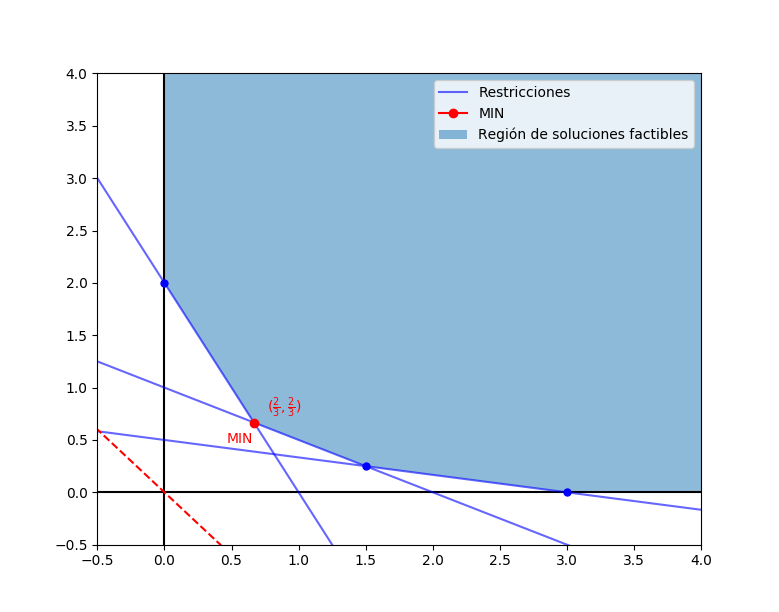
\includegraphics[width=\textwidth]{imagenes/ej2.png}
        \end{column}
        \begin{column}{0.3\textwidth}
            $\Rightarrow$ el mínimo se alcanza en $\yopt=(\frac{2}{3}, \frac{2}{3})$
        \end{column}
    \end{columns}
%    \end{figure}
%    \centering
\end{frame}

\begin{frame}{}
    Según el THC, debe valer que:
$$
\begin{array}{cclcc}
     \color<2>{Red}x_1^*=0 & \color<2>{Red}o & \color<2>{Red}2y_1^*+y_2^*=2 & \color<2>{Red}\text{(o ambas)} & \color<2>{Red}(1) \\
     \color<2>{Red}x_2^*=0 & \color<2>{Red}o & \color<2>{Red}y_1^*+2y_2^*=2 & \color<2>{Red}\text{(o ambas)} & \color<2>{Red}(2) \\
     \color<2>{Red}x_3^*=0 & \color<2>{Red}o & \color<2>{Red}\frac{1}{2}y_1^*+3y_2^*=\frac{3}{2} & \color<2>{Red}\text{(o ambas)} & \color<2>{Red}(3) \\
     y_1^*=0 & o & 2x_1^*+x_2^*+\frac{1}{2}x_3^*=18 & \text{(o ambas)} & (4) \\
     y_2^*=0 & o & x_1^*+2x_2^*+3x_3^*=15 & \text{(o ambas)} & (5) \\
\end{array}
$$
\end{frame}

\begin{frame}{}
    $$ y^*=(\frac{2}{3},\frac{2}{3})$$
    \pause
    \begin{tcolorbox}
        \centering
        $x_1^*=0 \quad o \quad 2y_1^*+y_2^*=2 \quad \text{(o ambas)} $
    \end{tcolorbox}

    
    \begin{align*}
        2y_1^*+y_2^*=2.\frac{2}{3}+\frac{2}{3}=2 \quad \text{\ding{51}}
    \end{align*}
    \pause
    \begin{tcolorbox}
    \centering
        $x_2^*=0 \quad o \quad y_1^*+2y_2^*=2 \quad \text{(o ambas)}   $ 
    \end{tcolorbox}

    \begin{align*}
        y_1^*+2y_2^*=\frac{2}{3}+2.\frac{2}{3}=2 \quad \checkmark
    \end{align*}
\end{frame}

\begin{frame}{}
    \begin{tcolorbox}
        \centering
        $x_3^*=0 \quad o \quad \frac{1}{2}y_1^*+3y_2^*=\frac{3}{2} \quad \text{(o ambas)}$    
    \end{tcolorbox}

    \begin{align*}
        \frac{1}{2}y_1^*+3y_2^*=\frac{1}{2}.\frac{2}{3}+3.\frac{2}{3}=\frac{7}{3}\neq\frac{3}{2} \quad \text{\alert{\ding{55}}}
    \end{align*}
    $$\Longrightarrow x_3^*=0$$
\end{frame}

\begin{frame}{}
        $$
\begin{array}{cclcc}
     x_1^*=0 & o & 2y_1^*+y_2^*=2 & \text{(o ambas)} & (1) \\
     x_2^*=0 & o & y_1^*+2y_2^*=2 & \text{(o ambas)} & (2) \\
     x_3^*=0 & o & \frac{1}{2}y_1^*+3y_2^*=\frac{3}{2} & \text{(o ambas)} & (3) \\
     \color{Red}y_1^*=0 & \color{Red}o & \color{Red}2x_1^*+x_2^*+\frac{1}{2}x_3^*=18 & \color{Red}\text{(o ambas)} & \color{Red}(4) \\
     \color{Red}y_2^*=0 & \color{Red}o & \color{Red}x_1^*+2x_2^*+3x_3^*=15 & \color{Red}\text{(o ambas)} & \color{Red}(5) \\
\end{array}
$$
\end{frame}

\begin{frame}{}
    \begin{tcolorbox}\centering
     $y_1^*=0 \quad o \quad 2x_1^*+x_2^*+\frac{1}{2}x_3^*=18 \quad \text{(o ambas)}$
    \end{tcolorbox}
    \begin{align*}
        y_1^*\neq0 \quad \Longrightarrow \quad 2x_1^*+x_2^*+\frac{1}{2}x_3^*=18
    \end{align*}
    
    \pause
    \begin{tcolorbox}
    \centering
    $    y_2^*=0 \quad o \quad x_1^*+2x_2^*+3x_3^*=15 \quad \text{(o ambas)}$
    \end{tcolorbox}
    \begin{align*}
        y_2^*\neq0 \quad \Longrightarrow \quad x_1^*+2x_2^*+3x_3^*=15
    \end{align*}
    
\end{frame}

\begin{frame}{}
    $$
    \begin{cases}
    2x_1^*+x_2^*+\frac{1}{2}x_3^*=18 \\ x_1^*+2x_2^*+3x_3^*=15
    \end{cases}
    \pause
    \xLeftrightarrow[]{x_3^*=0}
    \begin{cases}
    2x_1^*+x_2^*=18 \\ x_1^*+2x_2^*=15
    \end{cases}
    $$
    \pause
    $$\iff x_1^*=7 \quad \wedge \quad x_2^*=4$$
    \begin{center}
    $\color{Red}x^*=(7,4,0)$\\
    $\color{Red}z^*=22$ 
    \end{center}
\end{frame}

\begin{frame}{Dualidad}\footnotesize
    \begin{tcolorbox}[title=Teorema]
    Una solución factible $\xopt_1, \cdots, \xopt_n$ de 
    \[\begin{array}{rrl}
        \max & \multicolumn{2}{l}{\displaystyle\sum_{j=1}^n c_jx_j}  \\
        \text{s.a:} & \sum_{j=1}^n a_{ij}x_j \leq & b_i \qquad \forall i=1,\cdots,m \\
         & x_j \geq & 0 \qquad \forall j=1,\cdots, n
    \end{array}\]
    es óptima si y sólo si existen $\yopt_1,\cdots,\yopt_m$ tales que:
    \[\begin{array}{rclcl}
        \displaystyle \sum_{i=1}^m a_{ij}\yopt_i & = & c_j & \text{cuando} & \xopt_j>0  \\
        \yopt_i & = & 0 & \text{cuando} & \displaystyle\sum_{j=1}^n a_{ij}\xopt_j < b_i  
    \end{array}
    \]
    y tales que:
    \[\begin{array}{rcll}
        \displaystyle\sum_{i=1}^m a_{ij}\yopt_i & \geq & c_j & \quad \forall j=1,\cdots,n  \\
        \yopt_i & \geq & 0 & \quad \forall i=1,\cdots,m 
    \end{array}
    \]
    \end{tcolorbox}
\end{frame}

\begin{frame}{}
    Dada una solución factible de un problema lineal, el teorema anterior brinda una manera de chequear si es óptima. \\
    \textbf{Ejemplo}: supongamos que tenemos el siguiente problema lineal:
    \[\begin{array}{rrrrrrrrrrrrrr}
        \max & 18x_1 & - & 7x_2 & + & 12x_3 & + & 5x_4 & & & + & 8x_6 \\
        \text{s.a:} & 2x_1 & - & 6x_2& + & 2x_3 & + & 7x_4& + & 3x_5& + & 8x_6 &\leq & 1 \\ 
        & -3x_1 & - & x_2& + & 4x_3 & - & 3x_4& + & x_5& + & 2x_6 &\leq & -2 \\ 
        & 8x_1 & - & 3x_2& + & 5x_3 & - & 2x_4&  & & + & 2x_6 &\leq & 4 \\ 
        & 4x_1 &  & & + & 8x_3 & + & 7x_4& - & x_5& + & 3x_6 &\leq & 1 \\ 
        & 5x_1 & + & 2x_2& - & 3x_3 & + & 6x_4& - & 2x_5& - & x_6 &\leq & 5 \\
        & \multicolumn{11}{r}{x_1,x_2,x_3,x_4,x_5,x_6} & \geq & 0
    \end{array}
    \]
    Y queremos chequear si la siguiente solución es óptima:
    \[\xopt_1=2, \; \xopt_2=4, \; \xopt_3=0, \; \xopt_4=0, \; \xopt_5=7, \; \xopt_6=0 \]
\end{frame}

\begin{frame}{}
    % Queremos chequear si la siguiente solución es óptima:
    % \[\xopt_1=2, \; \xopt_2=4, \; \xopt_3=0, \; \xopt_4=0, \; \xopt_5=7, \; \xopt_6=0 \]
    Basta chequear que existan $\yopt_1,\cdots, \yopt_5$ que cumplan las hipótesis del teorema.
    Como $\xopt_1> 0$, $\xopt_2> 0$ y $\xopt_5> 0$, los $\yopt_i$ deben cumplir que:
    \[        \displaystyle \sum_{i=1}^m a_{ij}\yopt_i = c_j \quad \forall j\in\{1,2,5\} \]
    Es decir, deben cumplir que:
    \[\begin{array}{rrrrrrrrrrr}
        2\yopt_1 & - & 3\yopt_2 & + & 8\yopt_3 & + &4\yopt_4& + &5\yopt_5& = & 18\\
        -6\yopt_1 & - & \yopt_2 & - & 3\yopt_3 & & & + &2\yopt_5& = & -7\\
        3\yopt_1 & + & \yopt_2 &  &   & - & \yopt_4 & - &2\yopt_5& = & 0\\
    \end{array}
    \]
    Por otro lado:
    \[ \underbrace{-3\xopt_1  -  \xopt_2 + 4\xopt_3 - 3\xopt_4 +  \xopt_5 + 2\xopt_6}_{=-3} < -2 \Rightarrow \yopt_2=0\]
    \[\underbrace{5\xopt_1 + 2\xopt_2 - 3\xopt_3 + 6\xopt_4 -  2\xopt_5 - \xopt_6}_{=4} < 5 \Rightarrow \yopt_5=0    \]
\end{frame}

\begin{frame}{}
    Juntando todas las condiciones:
    \[\begin{array}{rrrrrrrrrrr}
        2\yopt_1 & - & 3\yopt_2 & + & 8\yopt_3 & + &4\yopt_4& + &5\yopt_5& = & 18\\
        -6\yopt_1 & - & \yopt_2 & - & 3\yopt_3 & & & + &2\yopt_5& = & -7\\
        3\yopt_1 & + & \yopt_2 &  &   & - & \yopt_4 & - &2\yopt_5& = & 0\\
         &  & \yopt_2 &  &   &   & &   & & = & 0\\
         &  &  &  &  &  & &   & \yopt_5& = & 0\\
    \end{array}
    \]
    La solución para este sistema es $(\frac{1}{3}, 0, \frac{5}{3}, 1, 0)$. Como esta solución verifica que:
        \[\begin{array}{rcll}
        \displaystyle\sum_{i=1}^5 a_{ij}\yopt_i & \geq & c_j & \quad \forall j=1,\cdots,6  \\
        \yopt_i & \geq & 0 & \quad \forall i=1,\cdots,5 
    \end{array}
    \]
    Entonces $\xopt$ es solución óptima.
\end{frame}

\end{document}


